\documentclass{article}
\usepackage{amsmath}
\usepackage{amssymb}
\usepackage{graphicx}
\usepackage{hyperref}
\usepackage[version=4]{mhchem}


\begin{document}
\section*{Problem}
(2017 Mathcounts National) In right triangle \(A B C\) with right angle at vertex \(C\), a semicircle is constructed, as shown, with center \(P\) on leg \(A C\), so that the semicircle is tangent to leg \(B C\) at \(C\), tangent to the hypotenuse AB , and intersects leg \(A C\) at \(Q\) between \(A\) and \(C\). The ratio of \(A Q\) to \(Q C\) is \(2: 3\). If \(B C=12\), then what is the value of \(A C\) ? Express your answer in simplest radical form.

\section*{Solution}
\(8 \sqrt{10}\).\\
We know that triangle \(A B C\) is a right triangle with right angle at vertex \(C\). The semicircle centered at \(P\) and is\\
\centering
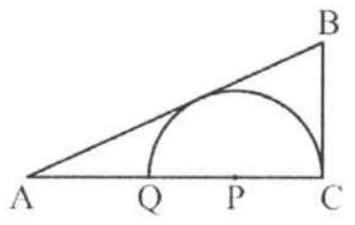
\includegraphics[width=\textwidth]{images/160(2).jpg}\\
tangent to leg \(B C\) at \(C\), tangent to the hypotenuse \(A B\). So \(B C=12\) and \(B D=12\).\\
Connect \(D P\). \(D\) is the tangent point as shown.\\
Since \(\frac{A Q}{Q C}=\frac{2}{3}, A Q=\frac{2}{3} Q C=\frac{2}{3} \times 2 r=\frac{4}{3} r\).\\
We want to find \(\frac{4}{3} r+r+r\).\\
Applying Pythagorean theorem to triangle \(A D P\) :\\
\centering
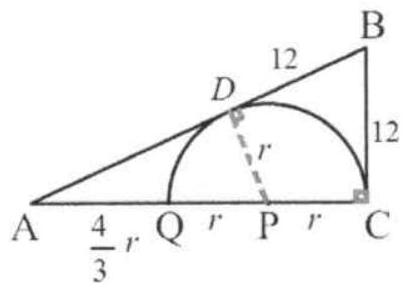
\includegraphics[width=\textwidth]{images/161(1).jpg}\\
\(A D=\sqrt{\left(\frac{4}{3} r+r\right)^{2}-r^{2}}=\sqrt{\left(\frac{4}{3} r+r\right)^{2}-r^{2}}=\frac{2 \sqrt{10}}{3} r\).\\
Since \(\triangle A B C \sim \triangle A P D, \frac{B C}{A C}=\frac{D P}{A D} \Rightarrow \frac{12}{\frac{4}{3} r+r+r}=\frac{r}{\frac{2 \sqrt{10}}{3} r}\)\\
\(\Rightarrow \quad \frac{12}{\frac{4}{3} r+r+r}=\frac{1}{\frac{2 \sqrt{10}}{3}} \quad \Rightarrow \quad \frac{4}{3} r+r+r=12 \times \frac{2 \sqrt{10}}{3}=8 \sqrt{10}\).

\end{document}
